\section{Representing Information}

\subsection{Electricity \& Information: Volts, Amps, \& Watts}
\label{sec:info}

\noindent
Figuring out how to represent information is tricky: Nature encodes information in DNA, though 
it may be hard to store because of decay (This is an active area of research). Punching holes 
in cards was a common method of storing information, but it's difficult to manipulate \cite{terman2017computation_structures}. Ideally:
\begin{itemize}
    \item \textbf{Inexpensive:} We want to reproduce at scale with low costs.
    \item \textbf{Stable:} Reliably store information for long periods.
    \item \textbf{Mutable:} The ability to manipulate information easily.
\end{itemize}

\begin{Def}[Electricity \& Information]

    \label{def:elec_info}

    Electricity is a flow of electrons, which can be used to represent information. 
    We can use the presence or absence of an electric current to represent binary values:
    \begin{itemize}
        \item \textbf{1} for presence of current;
        \item \textbf{0} for absence of current.
    \end{itemize}
    \noindent
    This is the basis of digital electronics and computing.
\end{Def}
\noindent
This is great for our applications, as electricity is relatively inexpensive given the scale of production.

\begin{theo}[Noise \& Error Accumulation]

    \label{theo:noise}

    We ought to keep in mind that electricity is not perfect. Though we design systems to measure information,
    slight inaccuracies or environmental factors may introduce noise, which over time corrupts information.
\end{theo}

\newpage 

\noindent
It's important that we understand the difference between analog and digital systems:
\begin{Def}[Analog vs. Digital Circuits]

    \label{def:analog_digital}

    A \textbf{circuit} is a closed path through which electricity flows, allowing us to manipulate and measure electrical signals.
    
    An \textbf{analog} system is one that uses continuous signals to represent information, while a \textbf{digital} system uses discrete values (e.g., binary) to represent information.
\end{Def}

\begin{Example}[Real World Analog vs. Digital]

    \noindent
    Vinyl records are analog, as the grooves on the record represent sound waves continuously. 
    In contrast, a digital system would be a CD or MP3 file, where sound is represented as discrete samples of the original sound wave.
\end{Example}

\noindent
Our main focus will be on digital systems, representing the strength of electricity as binary values.
First we will briefly understand the terminology used in electrical systems:
\begin{Def}[Voltage, Amps, \& Watts]

    \label{def:voltage_amps_watts}

    Definition wise we have the following terms in electrical systems:
    \begin{itemize}
        \item \textbf{Voltage (Volts):} The potential difference between two points in an electrical circuit, measured in volts (V).
        \item \textbf{Amperage (Amps):} The flow of electric \textbf{current}, measured in amperes (A/$I$).
        \item \textbf{Resistance (Ohms):} The opposition to the flow of electric current, are ohms ($\Omega$/R).
        \item \textbf{Power (Watts):} The rate at which electrical energy is transferred, are watts (W).
    \end{itemize}

    \noindent
    We calculate all such as follows:
    \begin{itemize}
        \item \textbf{Voltage:} $V = I \cdot R$ (Voltage = Current $\times$ Resistance).
        \item \textbf{Current:} $I = P / V$ (Current = Power / Voltage).
        \item \textbf{Resistance:} $R = V / I$ (Resistance = Voltage / Current).
        \item \textbf{Power:} $P = V \cdot I$ (Power = Voltage $\times$ Current).
    \end{itemize}

    \noindent
    These ratios between Voltage, Current, and Resistance are part of \textbf{Ohm's Law}.
\end{Def}

\newpage 

\noindent
Let's understand this with a common analogy to water flow:

\begin{Example}[Water \& Electric Flow Analogy]

    \noindent
    Imagine a water pipe system:
    \begin{itemize}
        \item \textbf{Voltage} is the water pressure in the pipes, the force pushing water through the system.
        \item \textbf{Current} is the amount of water flowing through the pipes at any given time.
        \item \textbf{Resistance} is the size of the pipes, which affects how easily water can flow.
        \item \textbf{Power} is the total amount of water that flowed through the system over time.
    \end{itemize}
\end{Example}


\noindent
The relationship between Voltage, Current, and Resistance has a handy visualization:

\begin{Def}[Ohm's Triangle]

    \label{def:ohms_triangle}

    \noindent
    Ohm's Triangle is a visual representation of the relationship between Voltage, Current, and Resistance. 
    If any two values are known, the third can be calculated using the triangle:\\

\noindent
    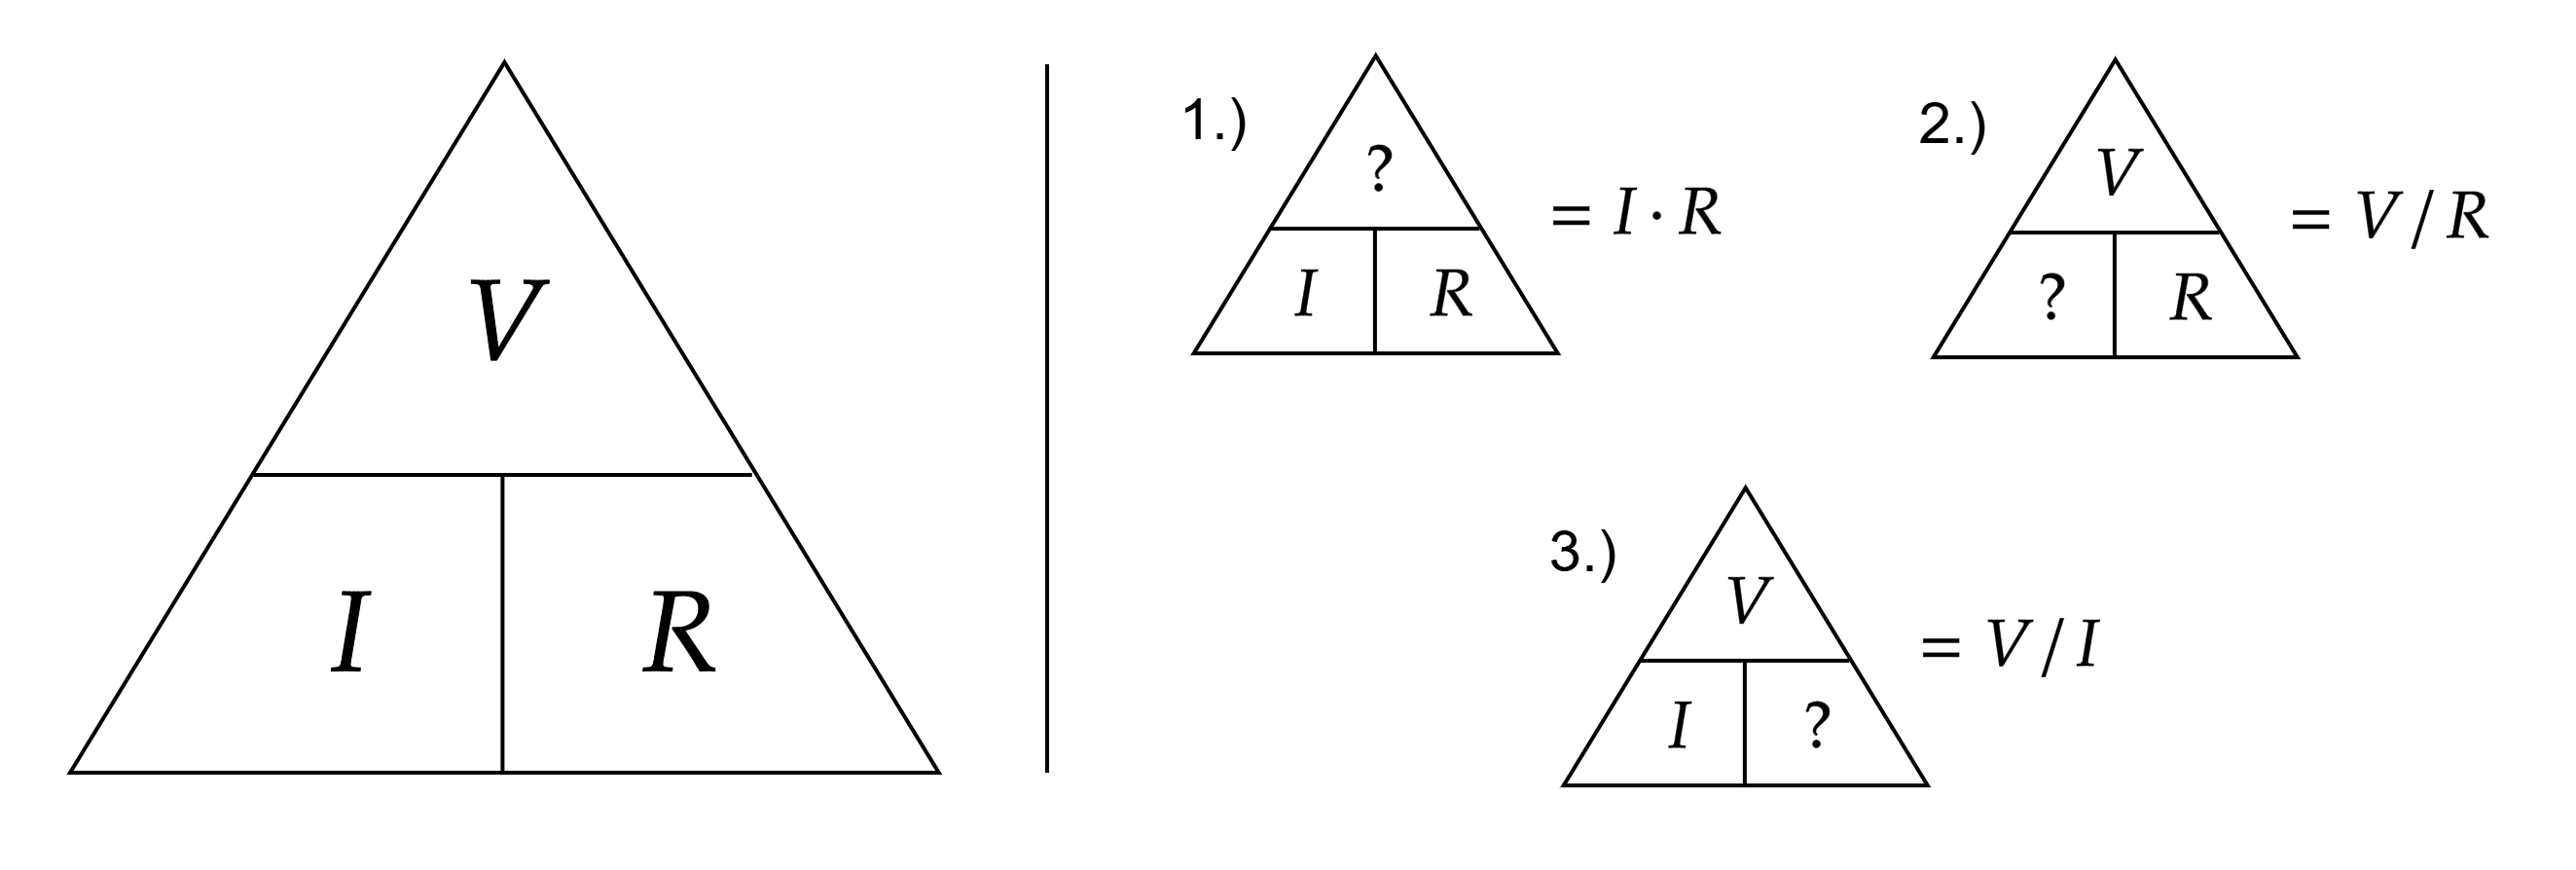
\includegraphics[width=\textwidth]{./Sections/circuits/triangle.png}

    \noindent
    Here, Voltage ($V$) is at the top, with Current ($I$) and Resistance ($R$) at the bottom corners:
    \begin{enumerate}
        \item \textbf{Voltage} is unknown: $V = I \cdot R$.
        \item \textbf{Current} is unknown: $I = V / R$.
        \item \textbf{Resistance} is unknown: $R = V / I$
    \end{enumerate}

    \noindent
    A common mnemonic to remember is ``Viral'' for VIR (Voltage, Current, Resistance).
\end{Def}

\newpage 

\noindent
Now for completeness sake, we distinguish the following:

\begin{Def}[Energy vs. Power]

    \label{def:energy_power}

    \noindent
    \textbf{Energy} is the capacity to do work, measured in joules (J). 
    \textbf{Power} is the rate at which work/energy is done or used, measured in watts (W).
    \noindent
    This is given by the formulation:
    \[
        P = E / t
    \]
    where $P$ is power, $E$ is energy, and $t$ is time.
\end{Def}

\noindent
\begin{Example}[Energy-Power Water Analogy]

    \noindent
    Continuing with the water analogy:
    \begin{itemize}
        \item \textbf{Energy} is the total amount of water stored in a tank.
        \item \textbf{Power} is how fast water flows out of the tank per second.
    \end{itemize}
    \noindent
    If we have a large tank (more energy), and water flows out slowly, we have high energy but low power. 
    Conversely, if we open the tap wide (high power), we use up the water quickly.

   
\end{Example}

\noindent
We will wrap up such with a final analogy that uses numbers:
 \begin{Example}[Mathematical Water Analogy]

        \begin{itemize}
            \item \textbf{Water Gun:} Imagine a water gun with very high pressure granted by
             the resistance of its small nozzle, so only a little water comes out.
            \begin{itemize}
                \item Pressure (Voltage) = 10 V
                \item Water Flow (Current) = 1 A
                \item Power = $10 \text{ V} \times 1 \text{ A} = 10 \text{ W}$
            \end{itemize}

            \item \textbf{Large Hose:} Now, consider a large fire hose with lower pressure but a much wider opening with 
            less resistance, allowing a lot of water to flow.
            \begin{itemize}
                \item Pressure (Voltage) = 2 V
                \item Water Flow (Current) = 5 A
                \item Power = $2 \text{ V} \times 5 \text{ A} = 10 \text{ W}$
            \end{itemize}
        \end{itemize}
        \noindent
        Both systems consumed the same amount of power (10 W), despite supporting different voltages, currents, and 
        possibly energy supplies. \textbf{Question:} What is the resistance of each system?

    \end{Example}

    \newpage 

    \subsection{Combinational Devices}

    \label{sec:digitally_encoding}

    \noindent
    We now focus on the conduits of representing information digitally:

    \begin{Def}[Digital Current Encoding Threshold]

        \label{def:digital_current_encoding_threshold}

        \noindent
        Given a line of voltage $V$, which we measure, $V_{TH}$ serves as a threshold:
        \[
         \text{0-bit} < V_{TH} < \text{1-bit}
        \]
        \noindent
        In practice, we have noise $\epsilon$ in our measurements, making it hard to 
        discern $V_{TH}+\epsilon$ from $V_{TH}-\epsilon$. To mitigate this, we
        pad the threshold from both sides called the \textbf{forbidden zone}:
        \[
        \text{0-bit} \leq V_{L} < \text{``Forbidden Zone''} < V_{H} \leq \text{1-bit}
        \]

        \noindent
        Where $V_L$ (low-level) and $V_H$ (high-level) are the region markers for valid voltage distinction.
    \end{Def}

    \vspace{-.5em}
    \begin{Def}[Combinational Device]

        \label{def:combinational_device}

        \noindent
        A \textbf{combinational device} is follows four specifications (spec.) called the, \textbf{static discipline}:

        \begin{itemize}
            \item \textbf{Input:} A set of input signals (i.e., measuring voltage levels).
            \item \textbf{Output:} A set of output signals (i.e., outputting voltage levels).
            \item \textbf{Functional Spec:} A mapping of all possible input combinations to an output value.
            \item \textbf{Timing Spec:} Detailing an upper bound $t_{PD}$ \textbf{(Propagation Delay)}, which is the minimum 
            amount of time needed for the output to stabilize on a new value after an input change.
        \end{itemize}
    \end{Def}

    \begin{figure}[ht!]

        \centering
        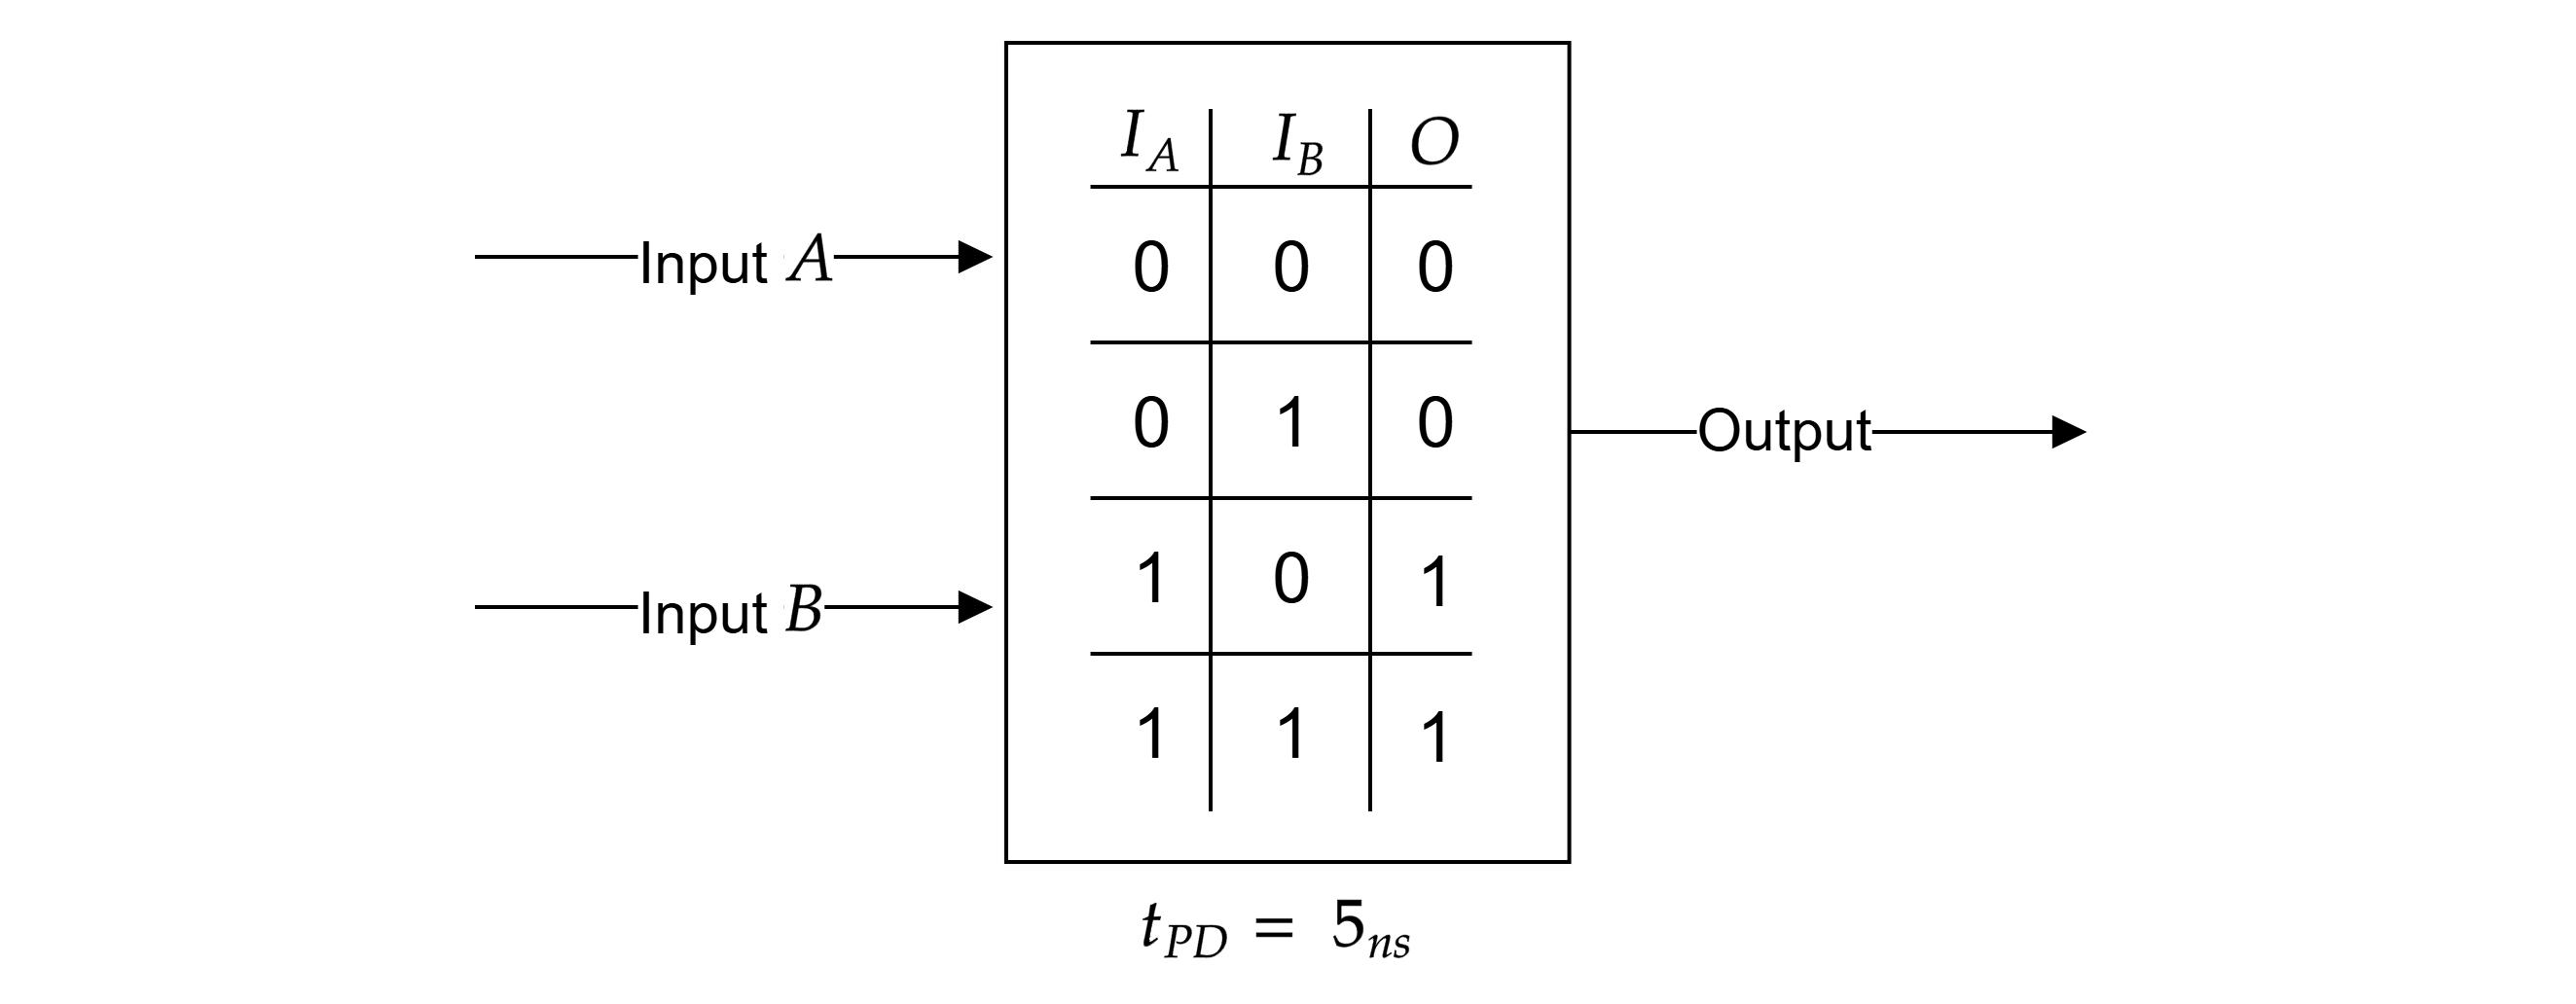
\includegraphics[width=.82\textwidth]{./Sections/circuits/combin.png}
        \caption{A combinational device with inputs $A$ and $B$, and a truth table detailing mappings towards the output.
        The $t_{PD}=5_{ns}$ (nanoseconds).}
        \label{fig:combinational_device}
    \end{figure}

    \newpage 

    \begin{Def}[Combinational Digital Systems]

        \label{def:combinational_digital_systems}

        \noindent
        A combinational device may also be made up of multiple other combinational devices. It must follow that:
        \begin{itemize}
            \item Each device is indeed a combinational device.
            \item Every input is connected to a single output.
            \item Each parent input will at most visit the same child input once (i.e., no cycles).
        \end{itemize}

        \noindent
        The $t_{PD}$ of the system is the sum of sub-devices $t_{PD}$'s along a path such that it is the 
        maximum such $t_{PD}$ path in the system.
    \end{Def}

    \vspace{-1em}

    \begin{figure}[ht!]

        \centering
        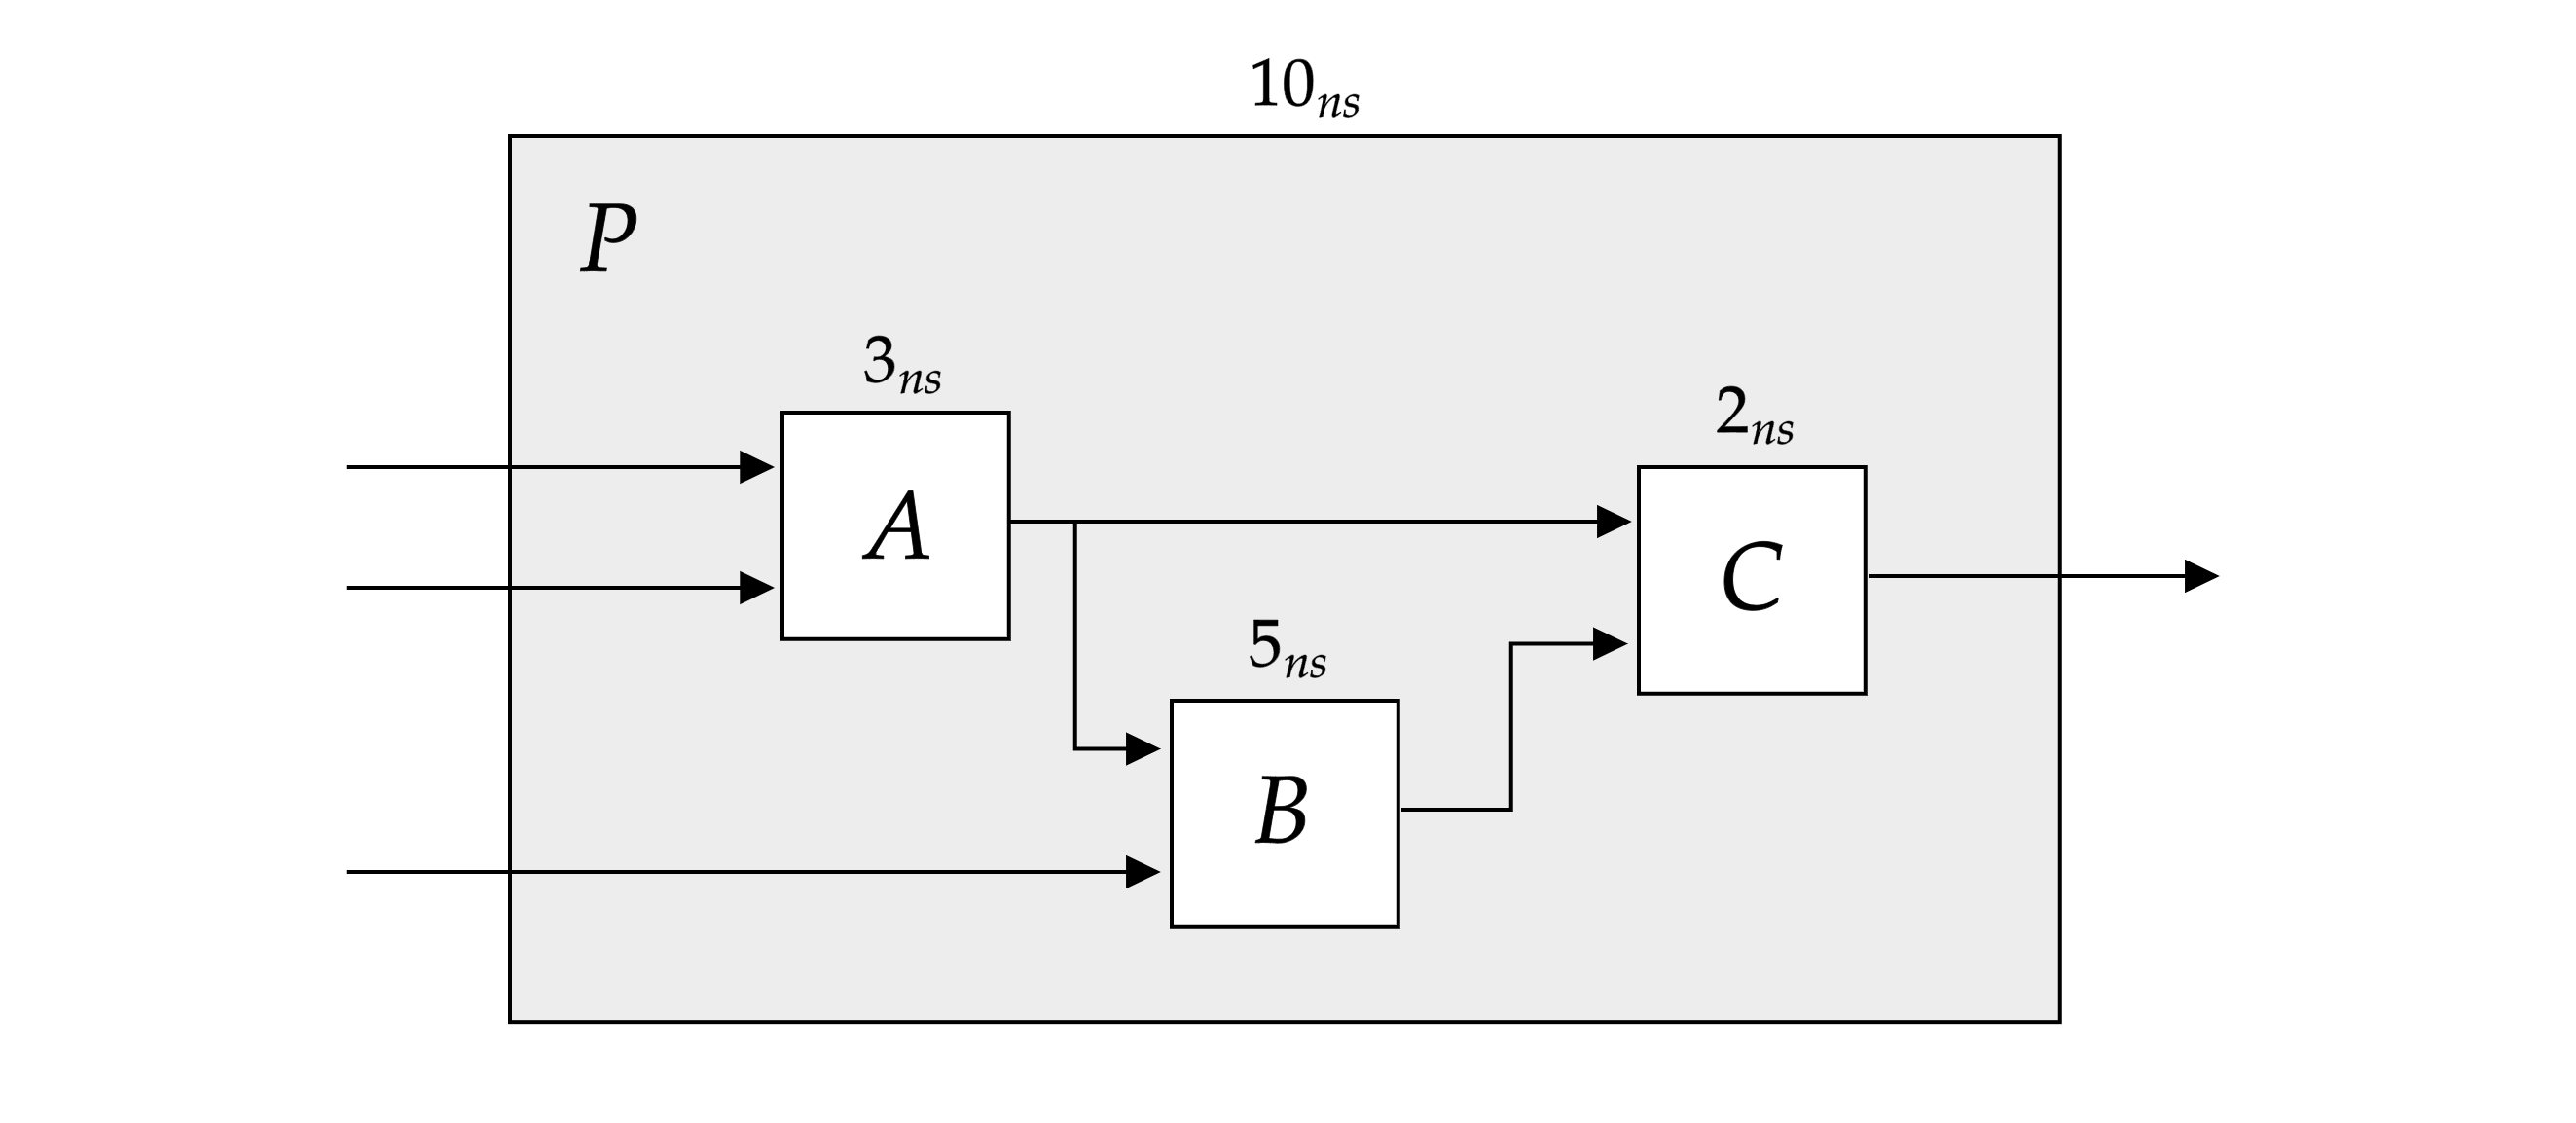
\includegraphics[width=.9\textwidth]{./Sections/circuits/combin_system.png}
        \caption{A combinational digital system, with a parent device $P$ and children devices $A,B$ and $C$.
        We abstract away the mappings focusing on the components and their connections. We see that there are no cycles and 
        all sub components are also combinational devices; Hence, the parent system is a combinational device. The 
        $t_{PD}$ of the system is $10_{ns}$, as the longest path takes $A\to B \to C = 3_{ns} + 5_{ns} + 2_{ns} = 10_{ns}$, the 
        effective bottleneck of the system.
        }
        \label{fig:combinational_digital_systems}
    \end{figure}

    \noindent
    Though this introduces a new problem:
    \begin{figure}[ht!]

        \centering
        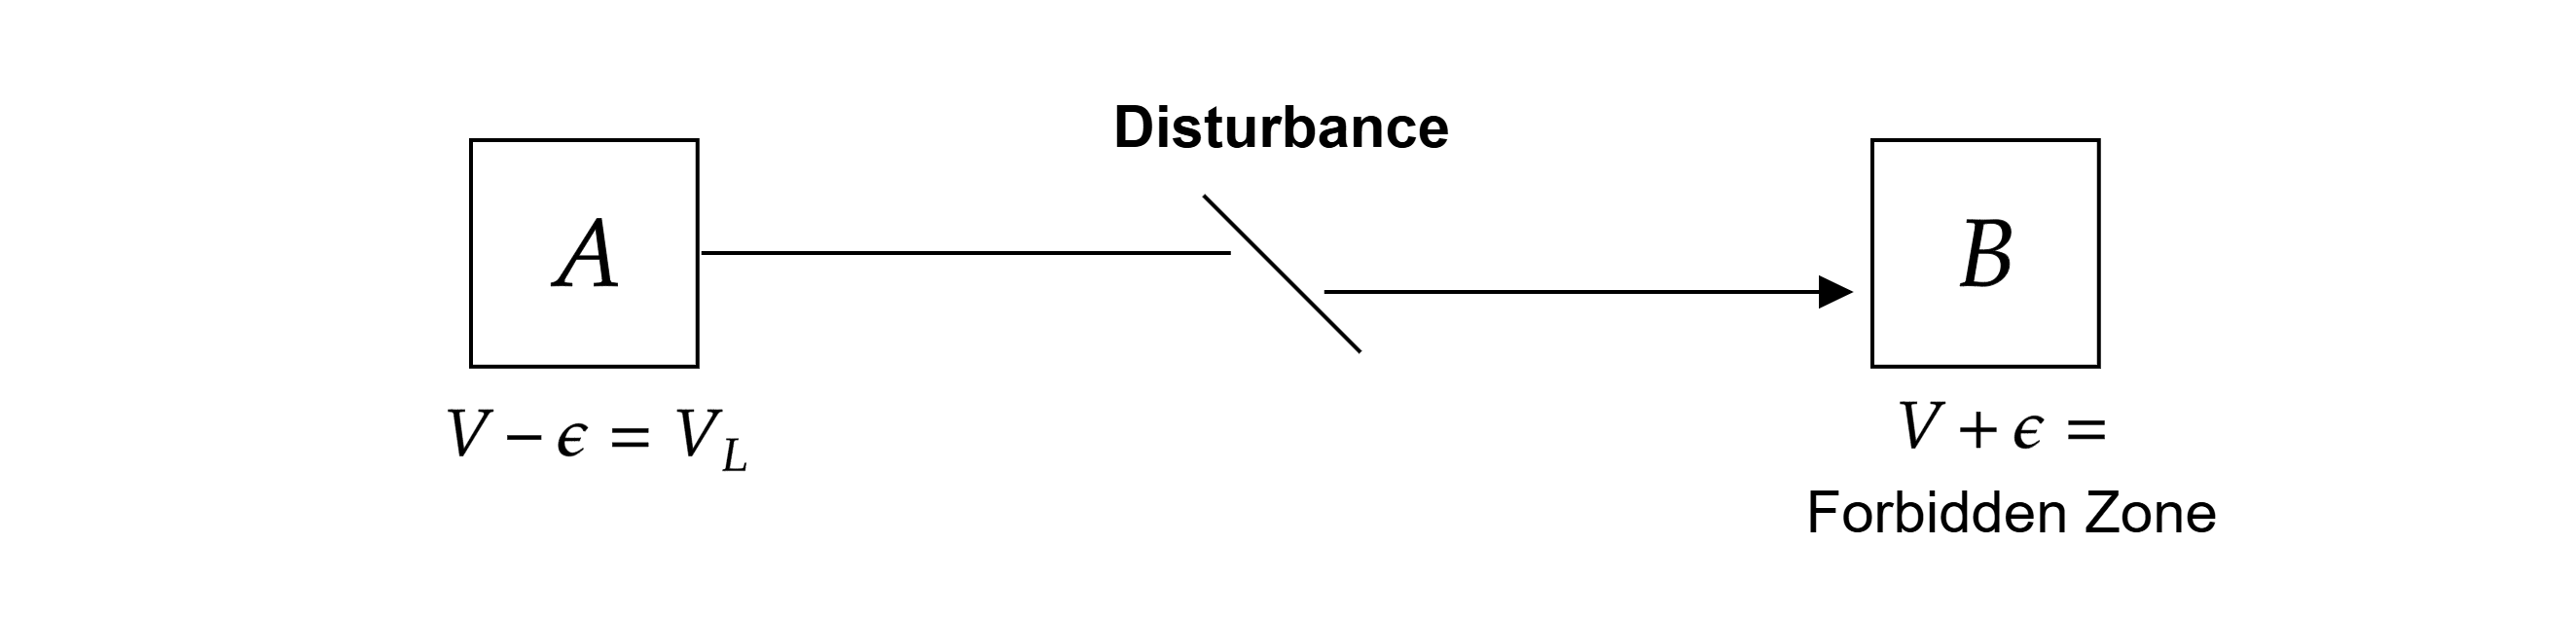
\includegraphics[width=.82\textwidth]{./Sections/circuits/combin_noise.png}
        \caption{Combinational devices $A$ and $B$ communicate; However, $A$'s output ($V$) is dangerously close 
        to $V_{L}$, over the wire there is a disturbance, causing the input of $B$ to enter the forbidden zone.}
        \label{fig:combinational_digital_systems_cycle}
    \end{figure}

    \newpage 

    \noindent
    We offer a simple fix to this problem, by loosening up the thresholds during certain phases:

    \begin{Def}[Noise Margins]

        \noindent
        To mitigate noise from outputs of a combinational device, we decrease the \emph{forbidden zone} (FZ) for the 
        receiving device. The overlap between the output's FZ and the input's FZ is called the \textbf{noise margin}.
        Concretely, we define the following:\\

        \noindent
        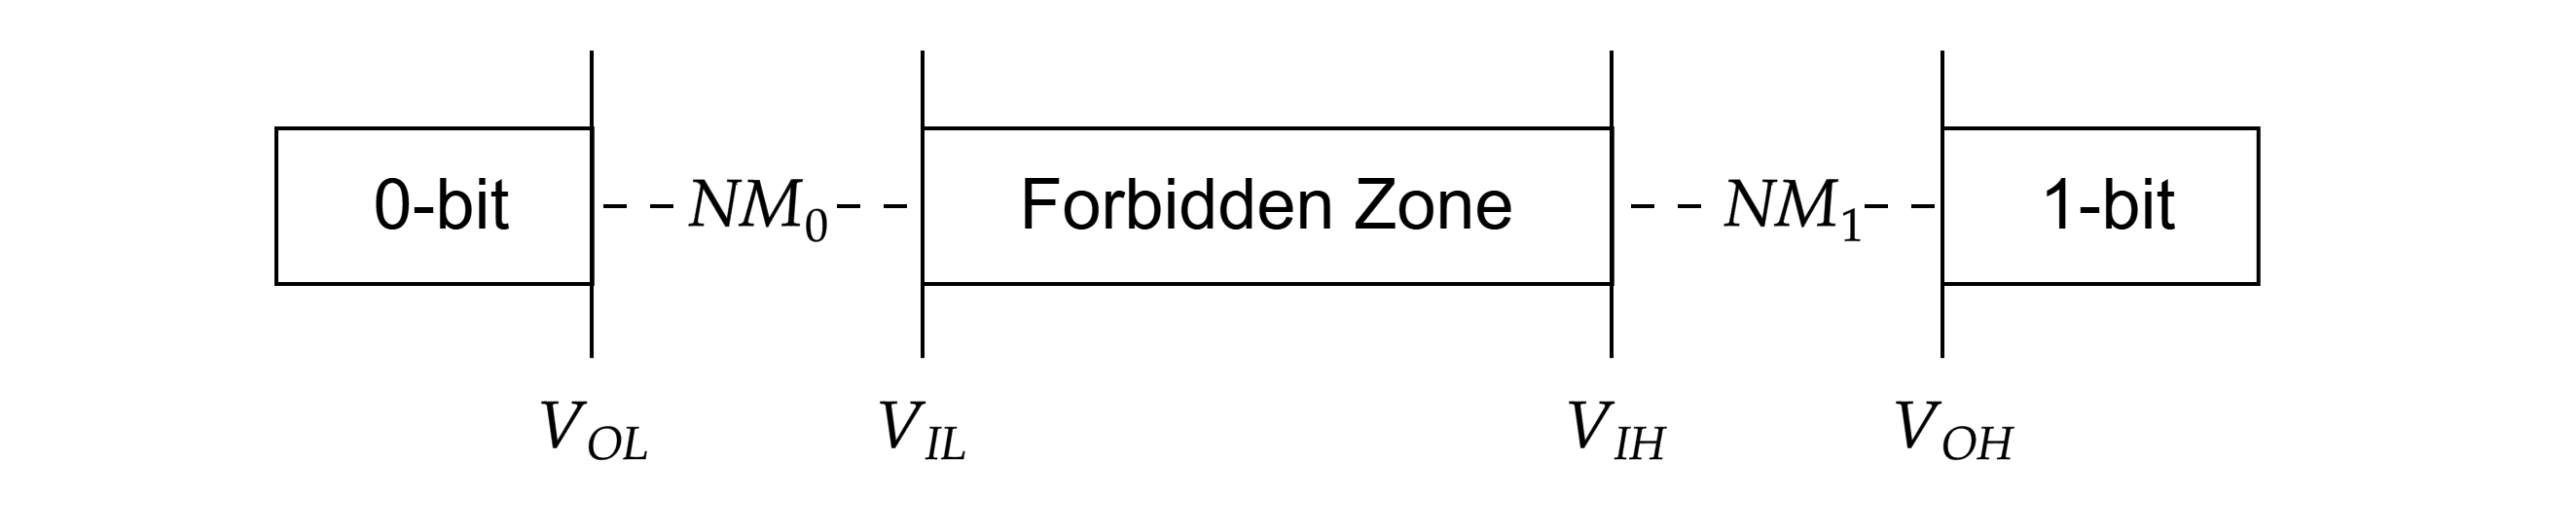
\includegraphics[width=\textwidth]{./Sections/circuits/noise_margin.png}

        \noindent
        Where, $V_{OL}$ and $V_{OH}$ are the output bounds, while $V_{IL}$ and $V_{IH}$ are the new input bounds.
        Then $\mathrm{NM}_0$ is the noise margin for the 0-bit, and $\mathrm{NM}_1$ is the noise margin for the 1-bit. The smallest 
        of the two is called the \textbf{noise immunity} of the device (i.e., the worst case that must be supported).
    \end{Def}


    \noindent
    Now when building our systems or combinational devices we must standardize how a particular device behaves on 
    inputs and outputs to account for the worst case noise.
    \begin{Def}[Voltage Transfer Characteristics (VTC)]

        \label{def:vtc}

        \noindent
        The \textbf{Voltage Transfer Characteristics} (VTC) is a graphical representation which shows how a device's inputs
        affect its outputs after stabilization. The horizontal axis measures the input voltage, while the vertical axis measures the output voltage.

        \begin{itemize}
            \item \textbf{Horizontal Axis ($V_{in}$):} Contains $V_{IL}$ and $V_{IH}$:
            \[V_{in} \leq V_{IL} \text{ (0-bit)} \quad \text{and} \quad V_{in} \geq V_{IH} \text{ (1-bit)}\]
            \noindent
            Otherwise, the input is in the forbidden zone.
            \item \textbf{Vertical Axis ($V_{out}$):} Contains $V_{OL}$ and $V_{OH}$:
            \[V_{OL} < \text{Invalid Outputs} < V_{OH} \quad \text{such that} \quad V_{in} < V_{OL}, V_{in} > V_{OH}\]
            \noindent
            I.e., if the input is already in the forbidden zone, the output is irrelevant.
        \end{itemize}

        \noindent
        It's given that the device must perform properly such that a $V_{in} > V_{IH}$ will always yield a $V_{out} > V_{OH}$, and a $V_{in} < V_{IL}$ will always yield a $V_{out} < V_{OL}$.
        Each device has its own VTC, plotting the input-output relationship. The resulting curve is the \textbf{VTC} of the device.
    \end{Def}

    \noindent
    \underline{Diagram next page.}

    \newpage

    \begin{figure}[ht!]

        \centering
        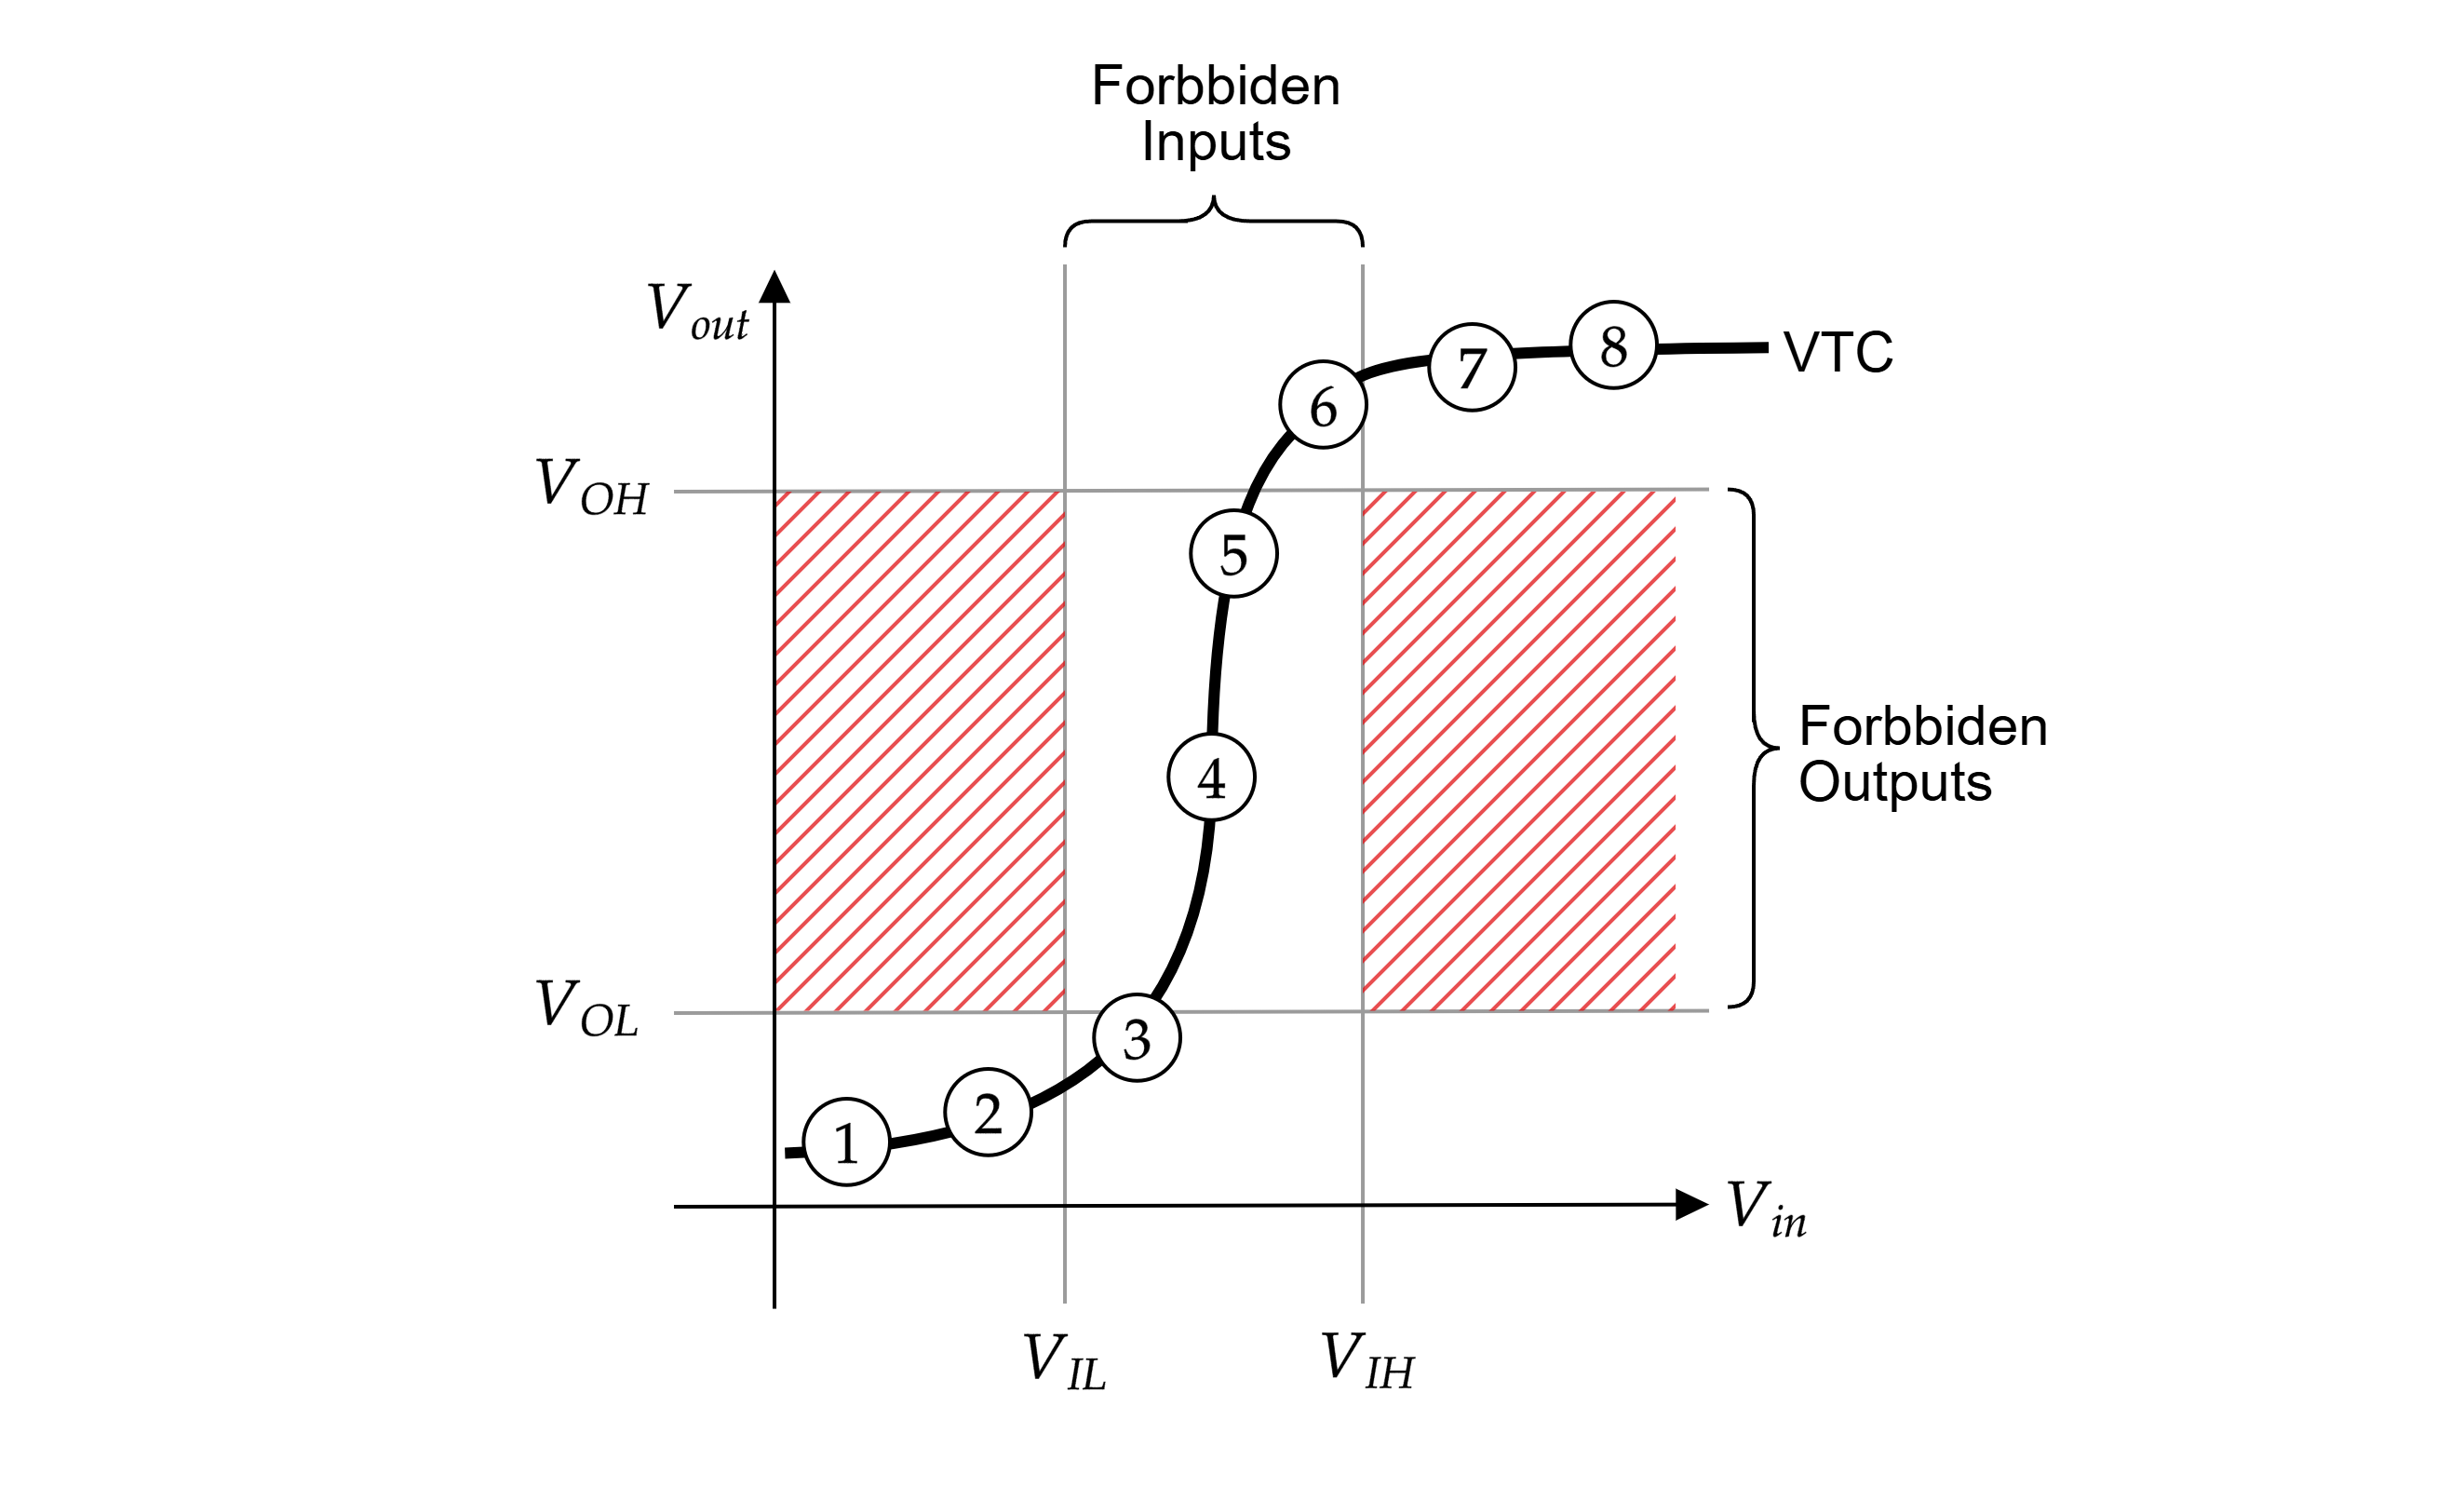
\includegraphics[width=\textwidth]{./Sections/circuits/vtc.png}
        \caption{A Voltage Transfer Characteristics (VTC) diagram, showing the input-output relationship of a device. 
        The horizontal axis represents the input voltage, while the vertical axis represents the output voltage. 
        The invalid output regions are shaded in red. The VTC is the bold line that crosses each point. Possible points: (1-2) received a
        low input and output reading, (3-6) undefined, and (7-8) high input and output reading. E.g., an inverter device (inverts logic) would be a vertical flip of the above VTC curve.}
        \label{fig:vtc}
    \end{figure}

    \noindent
    Notice how in Figure (\ref{fig:vtc}) the center white region is taller than it is wide:
    \begin{theo}[Properties of VTC -- Gain \& Nonlinearity]

    \label{theo:vtc_gain_nonlinearity}
    \noindent
    Since more leeway is allowed for input voltages, the following suffices $V_{OH} - V_{OL} > V_{IH} - V_{IL}$.
    We can compactly write this as:
    \begin{itemize}
        \item \textbf{Width of the transition (x-axis):} 
        $\Delta V_{in} = V_{IH} - V_{IL}$.
        \item \textbf{Height of the swing (y-axis):} 
        $\Delta V_{out} = V_{OH} - V_{OL}$.
    \end{itemize}

    \noindent
    Since $\Delta V_{out} > \Delta V_{in}$, the \textbf{gain} (average slope) satisfies:
    $
        \text{(avg.) gain}
        = \dfrac{\Delta V_{out}}{\Delta V_{in}}
        > 1.
    $

    \medskip

    \noindent
    Because of this ratio (gain $> 1$) small deviations (wiggles) in the input are amplified (exaggerated) in the output,
    which \textbf{regenerates} the signal (i.e., the output is a reinforced version of the input). The slope of the VTC
    must be \textbf{nonlinear} to ensure flat stable regions around 0 and 1 bits, and steep transitions between the forbidden zones (as seen in Figure \ref{fig:vtc}).
    \end{theo}
